% !TEX root = collection.tex

\newcommand{\eps}{\varepsilon}
\renewcommand{\inp}[1]{\left(#1\right)}
\newcommand{\inb}[1]{\left[#1\right]}
\newcommand{\inap}[1]{\left\langle #1\right\rangle}
\newcommand{\indi}[1]{\mathbbm{1}\inb{#1}}
\renewcommand{\abs}[1]{\left|#1\right|}
\renewcommand{\prob}[1]{\mathbb{P}\left[#1\right]}
\newcommand{\expec}[1]{\mathbb{E}\left[#1\right]}
\newcommand{\co}[1]{{\mathcal O}\left(#1\right)}
\newcommand{\tco}[1]{{\tilde{\mathcal O}}\left(#1\right)}
\renewcommand{\poly}[1]{{\sf poly}\left(#1\right)}
\newcommand{\polylog}[1]{{\sf polylog}\left(#1\right)}
\newcommand{\negl}[1]{\mathsf{negl}\inp{#1}}

\newcommand{\db}{D}
\newcommand{\odb}{\tilde D}
\renewcommand{\sk}{\mathsf{sk}}
\newcommand{\oram}{\mathsf{O}}
\newcommand{\oramdb}{\mathsf{DGen}}
\newcommand{\oramloc}{\mathsf{LGen}}
\newcommand{\secr}{\kappa}

\newcommand{\statInd}{\approx_s}

\chapter{Secure RAM Computation}

\section{Oblivious RAM}


Roughly speaking, an ORAM enables executing a RAM program while hiding the access pattern to the memory.
ORAM have several fundamental applications. For example, imagine a client has a huge memory/database $\db$. He wants to (encrypt and) store it on the server in such a way that later he can request and get access to a specific location of the database $\db[i]$ by communicating with the server without leaking any information of the location $i$ to the server.

\begin{definition}
An ORAM scheme $\oram = (\oramdb, \oramloc)$ consists of the following:
\begin{itemize}
  \item $\oramdb\inp{1^{\secr}, \db} \rightarrow \inp{\odb, \sk}$  given the security parameter and the initial database outputs an oblivious database and a secret key stored by the client, where $\abs{\sk} = \co{\polylog{\abs{\db}}}$.
  \item $\oramloc\inp{\sk, \ell_1, \cdots, \ell_T} \rightarrow \inp{\ell_1, \cdots, \ell_{T'}}$ given memory access locations of $\db$ outputs memory access locations of $\odb$. Note $T' = \co{T \cdot \polylog{\abs{\db}}}$.
\end{itemize}
Provided $\sk, \odb\inb{\ell_1}, \cdots, \odb\inb{\ell_{T'}}$ the client is able to recover $\db\inb{\ell_1}, \cdots, \db\inb{\ell_T}$.
Furthermore, for any $\inp{\ell_1, \cdots, \ell_T}$ and $\inp{\ell'_1, \cdots, \ell'_T}$ it satisfies
$$\oramloc\inp{\sk, \ell_1, \cdots, \ell_T} \statInd \oramloc\inp{\sk, \ell'_1, \cdots, \ell'_T}.$$
\end{definition}

In the following we first describe an ORAM construction where the client has storage of $\frac{n}{\alpha}$ for some constant $\alpha$, where $n$ is the size of $\db$. Then we will show this basic scheme suffices for constructing an ORAM scheme where the client has only $\polylog{n}$ storage.

\paragraph{A Basic Construction.}
Assume the client has storage of $\frac{n}{\alpha}$. First $\oramdb$ splits the database $\db$ into $\frac{n}{\alpha}$ blocks, each of size $\alpha$. Then it samples a ``position'' for each block uniformly at random from $\inb{\frac{n}{\alpha}}$, as in Figure~\ref{fig:position_map}. The position map is stored at the client.
\begin{figure}[h]
    \centering
    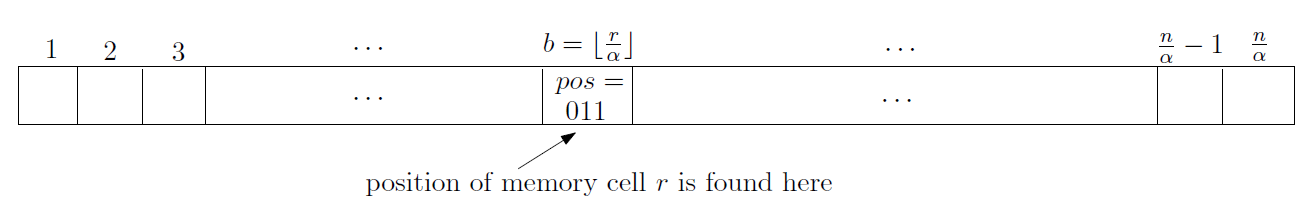
\includegraphics[scale = 0.48]{position_map.png}
    \caption{Position Map}
    \label{fig:position_map}
\end{figure}

An ORAM tree is then created as in Figure~\ref{fig:ORAM_tree}. It is a binary tree, each node in which is associated with a bucket which stores (at most) $K$ tuples $(b, pos, v)$ where $v$ is the content of block $b$ and $pos$ is the leaf associated with the block $b$. $K$ is a parameter that will determine the security of the ORAM.
\begin{figure}[h]
    \centering
    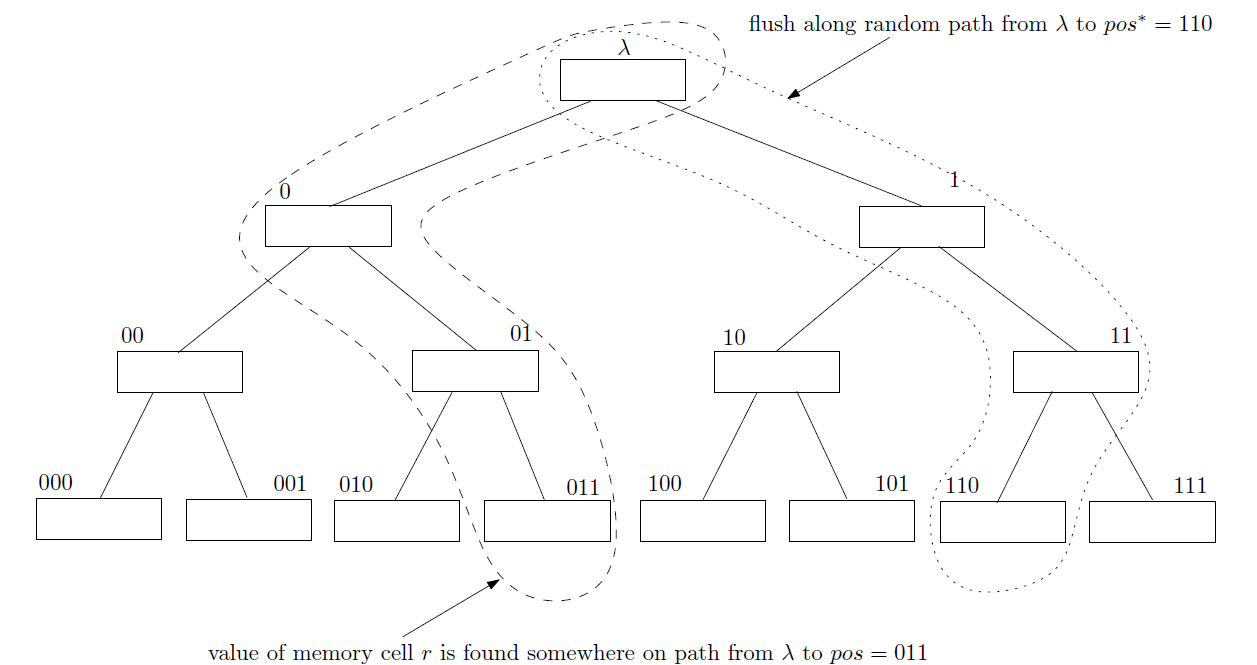
\includegraphics[scale = 0.5]{ORAM_tree.png}
    \caption{The ORAM Tree}
    \label{fig:ORAM_tree}
\end{figure}

When reading (or writing to) a memory block $b$, the client first requests the server for the entire path of $pos$ in the ORAM tree, then generates a new random position $pos'$ for $b$, deletes the old tuple $(b, pos, v)$ from the path, adds to the root a new tuple $(b, pos', v\text{(or $v'$)})$, and sends the entire path back to the server. After this, there is a \emph{flush} step, in which the client requests for a random path, and pushes each tuple in the path down as far as possible.


\paragraph{Security Proof.}
It is clear that the access patterns are hidden in the above construction, since every read/write/flush requests a uniformly random path. We only need to argue that the probability of \emph{overflow} (meaning that at any time a node in the ORAM tree contains more than $K$ tuples) is negligible.

Consider a dart game: you have an unbounded number of white and black darts. In each round of the game, you first throw a black dart, and then a white dart; each dart independently hits the bullseye with probability $p$. You continue the game until at least $K$ darts have hit the bullseye. You ``win'' if none of darts that hit the bullseye are white. The winning probability is upper bounded by $2^{-K}$.

Suppose there is a tree node $\gamma$ containing more than $K$ tuples at some point of time. Among the $K$ tuples at $\gamma$, WLOG assume at least $K/2$ tuples has $pos$ with prefix $\gamma||0$.
Think of black darts hitting bullseye as assigning a memory block to a leaf $pos$ with prefix $\gamma||0$, and white darts hitting bullseye as performing a flushing associated with a leaf $pos$ with prefix $\gamma||0$. By the union bound the probability of overflow is upper bounded by $T2^{-K}$.


\paragraph{The Full Scheme.}
Given an ORAM scheme where the client has storage of size $\frac{n}{\alpha}$ for some constant $\alpha$, the client can apply ORAM again on the smaller memory of size $\frac{n}{\alpha}$. After $\log(n)$ iterations, the client ends up needing storage of size $\polylog{n}$.



